\documentclass[10pt,a4paper]{report}

\usepackage[utf8]{inputenc}
\usepackage{amsmath}
\usepackage{amsfonts}
\usepackage{amssymb}
\usepackage{graphicx}
\usepackage{color}
\usepackage{enumitem}
\usepackage[top=1cm, bottom=2cm, left=2cm, right=2cm]{geometry}

\usepackage{fancyhdr}
\pagestyle{fancy}

\fancyhead{}
\fancyfoot{} 
\lhead{
\includegraphics{../Logo/logoKNKMini.jpg} \hspace{0.1cm} Kould Not Konect  \hspace{0.4cm} \vline}
\chead{Document de Conception Générale}
\rhead{Kould Not Share}
\rfoot{\thepage}

\author{Kevin BASCOL, Kevin LAOUSSING, Nicolas REYNAUD}
\title{Document de conception détaillé}
\date{24 Novembre 2014}

\makeatletter
\renewcommand{\thesection}{\@arabic\c@section}
\makeatother

\begin{document}

\makeatletter
	\begin{titlepage}
	
	\begin{figure}
		\begin{minipage}[c]{.46\linewidth}
		\end{minipage} \hfill
		\begin{minipage}[c]{.20\linewidth}
			\begin{center}
				
\includegraphics{../Logo/logoKNK.jpg}\\
				{\large Kould Not Konect}
			\end{center}
		\end{minipage}
	\vspace{1cm}
	\end{figure}
	
	\centering
		{
		\hrule height 2pt
		\vspace{0.7cm}
		\Huge \textbf{\@title}}\\
		\vspace{0.7cm}
		\hrule height 2pt
		\vspace{1.5cm}
		{\LARGE  Projet \textbf{Kould Not Share} v1.0}
		
		\vfill
		
		\begin{tabular}{|c|c|c|}
			\hline
			Version & Date & Description\\
			\hline
			V.1 & 16/11/14 & Première version de la conception générale\\
			\hline
			 & & \\
			\hline
			 & & \\
			\hline
		\end{tabular}\\
		\vspace{1cm}
		\@author\\
		\end{titlepage}
\makeatother
\setcounter{secnumdepth}{5}
\setcounter{tocdepth}{5}
\renewcommand{\contentsname}{Sommaire}
\begingroup\makeatletter
\def\@makeschapterhead#1{%
  {\parindent \z@ \raggedright
    \normalfont
    \interlinepenalty\@M
    \Huge \bfseries  #1\par\nobreak
    \vskip 20pt% <---- à réduire pour avoir plus de place
  }}\makeatother
\tableofcontents
\endgroup
\thispagestyle{empty}
\setcounter{page}{0}
\newpage

\newgeometry{top=2cm, bottom=2cm, left=2cm, right=2cm}

\section{Introduction}


\subsection{Portée du document}
Le logiciel de client/serveur FTP est un outil permettant à des particuliers ou des entreprises l'échange de donnée de manière contrôlée. Par exemple, chaque utilisateur propriétaire d'un fichier stocké dans le serveur FTP du logiciel, pourra paramétrer les droits de téléchargements sur ce fichier, et ainsi il disposera du pouvoir de restreindre ou d'augmenter l'accessibilité de son fichier...

\subsection{Objectif du document}

\subsection{Définitions, acronymes et abréviations}
\begin{description}
\item[KNK] Kould Not Konect.
\item[KNS] Kould Not Share.
\item[FTP] File Transfer Protocol, protocole de communication destiné à l'échange informatique de fichiers sur un réseau TCP/IP.
\item [MVC] : Modèle-Vue-Controleur, est un modèle destiné à répondre aux besoins des applications interactives en séparant les problématiques liées aux différents composants au sein de leur architecture respective.
\item[Protocole] Spécification de plusieurs règles pour un type de communication particulier.
\item[Client] Logiciel qui envoie des demandes à un serveur.
\item[Serveur] Dispositif informatique matériel ou logiciel qui offre des services, à différents clients.
\item[Downloader] Anglicisme du mot "télécharger".
\item[Uploader] Anglicisme du mot "téléverser".
\end{description}


\section{Description générale}

Ce projet consiste en la création d'un serveur FTP chez un particulier ou une entreprise, ayant accès à la machine sur laquelle est installé le programme. Les utilisateurs se verront donner l'accès par l'administrateur à certains dossiers de la machine sur laquelle est installé le serveur. Ils pourront faire alors des échanges de fichiers dans ces répertoires à l'aide du client FTP.\\

\newpage

\section{Architecture du système Kould Not Share}
Nous allons préciser les modules décrit dans le document de conception générale grâce à des diagrammes de classe.
\subsection{Module de gestion des dossiers}
Module décrit dans la section 3.1.2.1.3 du DCG.
\begin{center}
	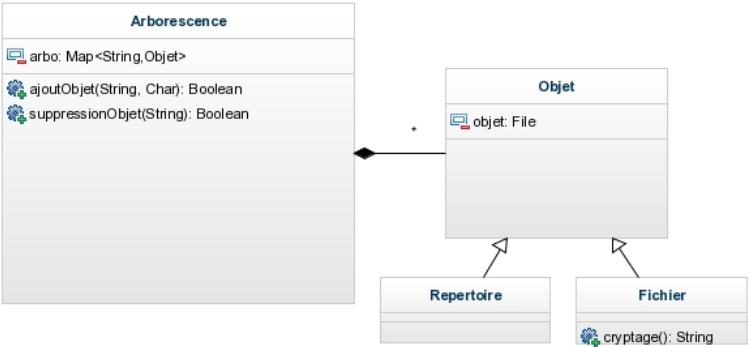
\includegraphics[scale=0.5]{./Ressources/modules_doss.png}\\
\end{center}

\hspace{5cm}

\subsection{Module de configurations et limitations}
Module décrit dans la section 3.1.2.1.4 du DCG.
\begin{center}
	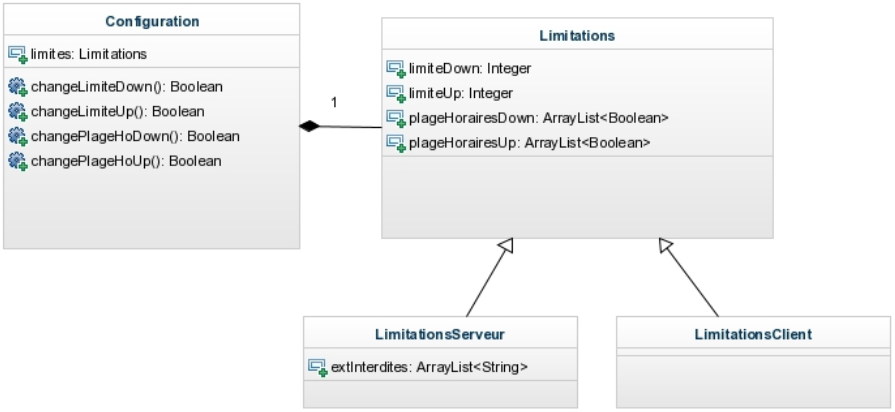
\includegraphics[scale=0.5]{./Ressources/modules_lim.png}\\
\end{center}

\newpage

\subsection{Module de communication}
Module décrit dans la section 3.1.2.1.7 du DCG.
\begin{center}
	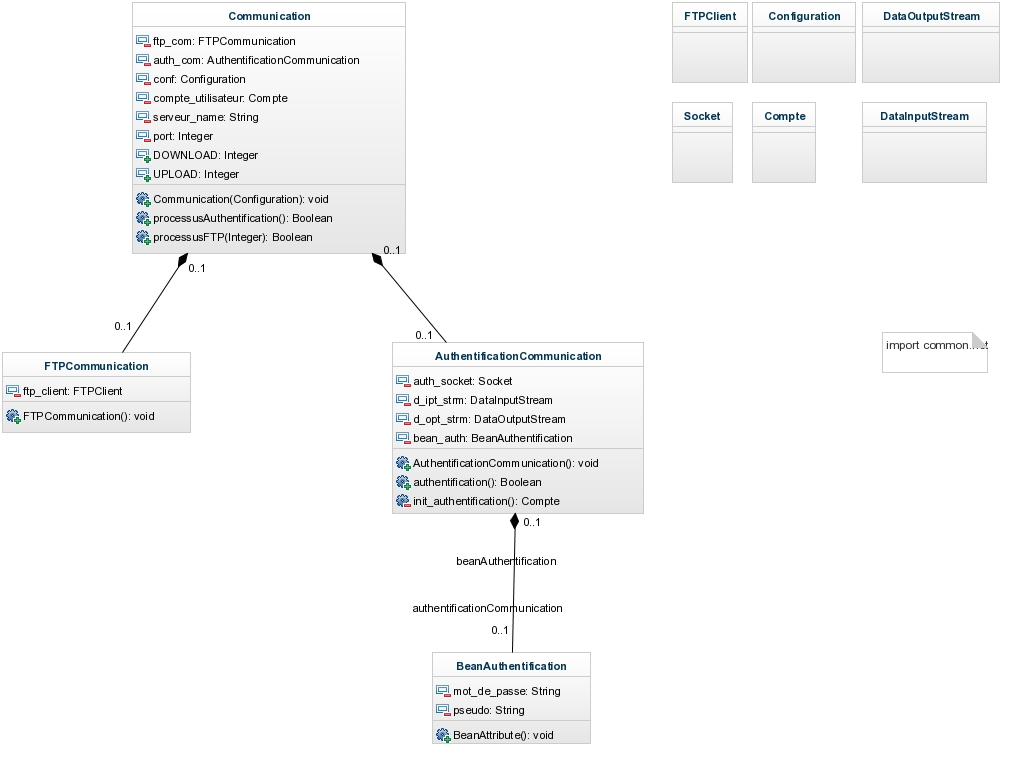
\includegraphics{./Ressources/communication.jpeg}\\
\end{center}

\newpage

\subsection{Module d'upload et download}
Module décrit dans la section 3.1.2.1.5 du DCG.
\begin{center}
	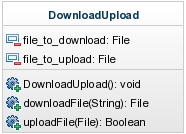
\includegraphics{./Ressources/downlaodUpload.jpeg}\\
\end{center}

\hspace{5cm}

\subsection{Module de statistiques}
Module décrit dans la section 3.1.2.1.6 du DCG.
\begin{center}
	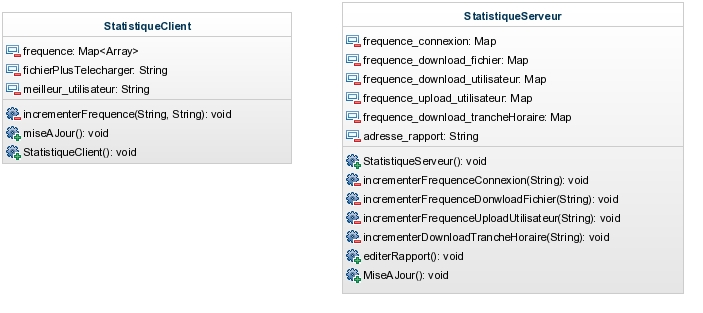
\includegraphics{./Ressources/statistique.jpeg}\\
\end{center}

\hspace{5cm}

\subsection{Module des historiques des événements}
Module décrit dans la section 3.1.2.2.1 du DCG.
\begin{center}
	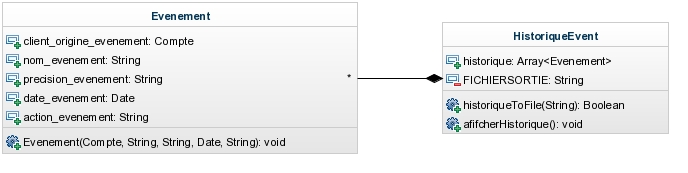
\includegraphics{./Ressources/historiqueEvenement.jpeg}\\
\end{center}

\newpage



\subsection{Module de gestion des comptes}
Module décrit dans la section 3.1.2.2.2 du DCG.
\begin{center}
	\rotatebox{90}{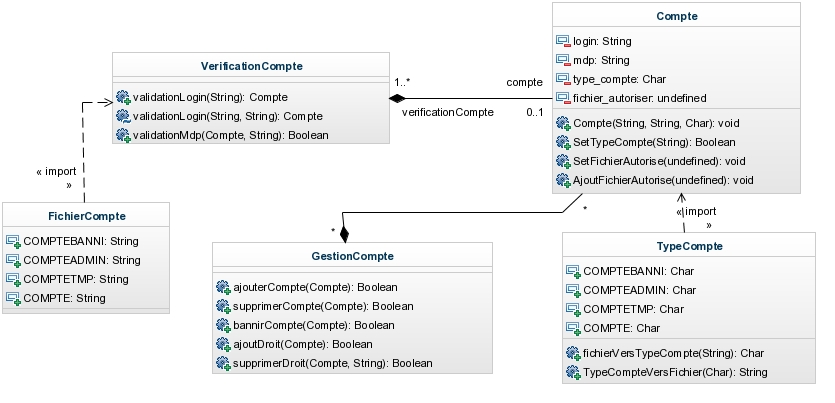
\includegraphics{./Ressources/gestionCompte.jpeg}}\\
\end{center}

\end{document}